\documentclass[sigconf]{acmart}

\AtBeginDocument{%
  \providecommand\BibTeX{{%
    \normalfont B\kern-0.5em{\scshape i\kern-0.25em b}\kern-0.8em\TeX}}}

\usepackage{dblfloatfix}
\usepackage{mathtools}
\usepackage{hyperref}

\begin{document}

\title{Information retrieval and Text Mining : Group Project}

% AUTHORS:
\author{Til Mohr}
\affiliation{}
\email{tv.mohr@stud.uis.no}

\author{Ishaac Ourahou}
\affiliation{}
\email{i.ourahou@stud.uis.no}

% DATE:
\date{\today}



\begin{abstract}
As part of our master's degree, we study information retrieval and text mining. This group project aims to design a system that addresses the problem of searching for passages within a conversation. This therefore consists of taking the context of the previous conversation history into account of the current user query, rewriting the current user query in a way that encompasses the conversation topic, selecting the most relevant passages to that rewritten query, through a collection of 8.8 million documents (MS MARCO passages). Based on the knowledge acquired on the subject, we present a baseline information retrieval pipeline, which will serve as our reference system for future comparisions with more advanced information retrieval pipelines. Afterwards, we dive into more advanced approaches in this field of conversational search engines. Finally, we make comparisons between the baseline system and the implemented advanced retrieval pipelines to highlight the positives and negatives of our implementations, and also draw conclusions.
\end{abstract}

\keywords{information retrieval, conversational search engine, conversational search system}

%% Remove copyright footer
\settopmatter{printacmref=false}
\setcopyright{none}
\renewcommand\footnotetextcopyrightpermission[1]{}
\pagestyle{plain}
%% ------------------------

%%
%% This command processes the author and affiliation and title
%% information and builds the first part of the formatted document.
\maketitle


\section{Introduction}\label{sec:intro}
Nowadays, we can see a strong development of conversational agents like Amazon Alexa or Apple Siri. These conversational agents aim to communicate with a user and return relevant responses to the requests that the user formulates. The need to return the right information is important to ensure the quality of the responses sent to the user.

The goal of our project is to create a conversational search engine, i.e. a system where the user may ask multiple questions (queries), and the system takes the conversation history, e.g. the current topic of the conversation, as well as the current query into accout to determine the most relevant documents to the user. We will design a simple basic architecture which will serve as our baseline system for future comparision with more advanced approaches. However, as a hard requirement, this baseline retrieval pipeline must already perform at least as well as the reference system provided by our project owners.

For this project, we will use the MS MARCO dataset, which contains 8.8 million documents. This document collection has to be indexed in order to be able to retrieve relevant documents efficiently. This indexing will be achieved through the \texttt{pyterrier} API.

In section \ref{sec:problem} we will define the problem statement at hand. Following the problem statement, we will dive into the implementation of the different retrieval pipelines we have developed. In general, retrieval pipelines can be segmented into the following stages: Query rewriting, (multi-pass) retrieval, reranking. In sections \ref{sec:baseline} and \ref{sec:advanced}, we will present our baseline and advanced retrieval pipelines in aspects of these components, respectively. Finally, in section \ref{sec:results}, we will present the performance results of our retrieval pipelines and compare them to each other, highlighting any improvements and drawbacks of our advanced retrieval pipelines.

\section{Problem Statement}\label{sec:problem}
The goal of this project is to design a conversational search engine (CSE). The main differeation of such a system to a ordinary search engine is that queries asked by the same user within a session are not independent of each other in a CSE. A CSE takes currently and past discussed topics into account for searching relevant passages. The system should be able to respond to queries which continue the flow of the conversation, as well as handle abrupt changes in the conversation topic. For each query, the system should then return a ranked list of the top 1000 most relevant passages from a collection of 8.8 million documents.

In addition to the components of a ordinary search engine retrieval pipeline, a CSE retrieval pipeline should also include a query rewriting component that rewrites the current query to reflect the current conversation topic. A overview of how the different components of a CSE retrieval pipeline interact with each other is shown in figure \ref{figure:global_pipeline}. As it is common practice in ordinary search engines, also in CSE the document collection must be indexed beforehand to facilitate efficient document retrieval and ranking.

\begin{figure}[h]
	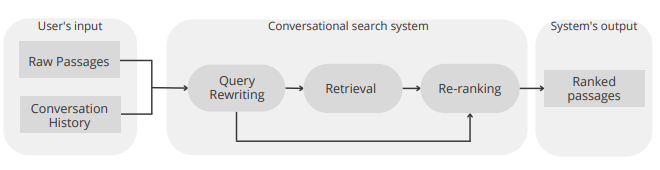
\includegraphics[width=7cm]{pipeline.png}
	\caption{Global Pipeline architecture of the system}
	\label{figure:global_pipeline}
\end{figure}


\section{Baseline Method}\label{sec:baseline}
Explain what you are taking as your baseline method, as well as why this is a reasonable baseline, and why you are making specific implementation choices.

Our baseline method is inspired by the baseline method presented by Łajewska et al. \cite{Lajewska:2023:ECIR}. Our baseline method consists of the following stages:
\begin{enumerate}
	\item	\texttt{T5} Query Rewriting
	\item	\texttt{BM25} Retrieval
	\item	Re-ranking
			\begin{enumerate}
				\item	Re-ranking with \texttt{monoT5}
				\item	Re-ranking top documents with \texttt{duoT5}
			\end{enumerate}
\end{enumerate}

\subsection{T5 Query Rewriting}
In conversation search engines, query rewriting is the crucial component to include the semantics of the conversation history into the currently asked query, which results into a singular rewritten query that can be passed along into the retrieval pipeline.

For this purpose, we include all the previously rewritten queries $q'_0 \dots q'_{n-1}$ of our conversation, as well as the response $r_{n-1}$ of the CSE to the previous rewritten query $q'_{n-1}$ into the current query $q_n$. This is done by concatenating the previous rewritten queries and the response into a single string:
\begin{align*}
	q'_n \coloneqq q'_0 \text{<sep>} \dots \text{<sep>} q'_{n-1} \text{<sep>} r_{n-1} \text{<sep>} q_n
\end{align*}
This approach resembles the approach taken by Łajewska et al. \cite{Lajewska:2023:ECIR}.

We have found through experimentation that this concatenation is insufficient to produce satisfiable results: The concatenated string is too long, and too much focus during the later retrieval is being put on $r_{n-1}$, which make sudden changes in topic impossible.

For those reasons, we have turned our attention to other query rewriting methods, which we could append to the currently followed approach. \texttt{Pyterrier} provides the \texttt{SequentialDependence} query rewriting method\footnote{URL: \url{https://pyterrier.readthedocs.io/en/latest/rewrite.html\#sequentialdependence}}. We have found, however, that this rewriter does not produce the desired result.

Researching further, we stumbled upon the \texttt{T5} neural query rewriter trained on conversational question rewriting\footnote{URL: \url{https://huggingface.co/castorini/t5-base-canard}}. This method produced the desired results: The rewritten query $q'_n$ resembles the original query $q_n$, just rewritten very slightly to include the conversation topic, if no sudden change was detected. As a side effect, the rewritten query is now also very small in size, and not growing with the number of queries asked in the conversation, as we saw in the previous approach.

\subsection{BM25 Retrieval}
The \texttt{BM25} retrieval method is a common retrieval method in information retrieval. We chose to use this retrieval method, as the reference system also uses this basic retrieval method. This allows us to easily compare our baseline system to the reference system.

\subsection{Re-ranking}
The re-ranking stage of our baseline system consists of two stages: First, the top 1000 documents retrieved by the \texttt{BM25} retrieval method are re-ranked using the \texttt{monoT5} reranker. Afterwards, the top 50 documents of the previous re-ranking stage are re-ranked using the \texttt{duoT5} reranker. The actual number of documents to be reranked in each stage is a hyperparameter of our system, and can be adjusted to trade off runtime and quality of the result. The rerankers were implemented in the \texttt{pyterrier\_t5} library.\footnote{URL: \url{https://github.com/terrierteam/pyterrier_t5}}


\section{Advanced Method}\label{sec:advanced}
Explain what you are taking as your advanced method(s), as well as why this is a promising attempt to outperform the baseline method, and why you are making specific implementation choices.

\section{Results}\label{sec:results}
The individual methods were evaluated on the MS MARCO document collection and the following provided files: \texttt{queries\_train.csv} holds a list of queries grouped together into several conversation sessions, and \texttt{qrels\_train.txt} contains the relevance assessments for the training queries. Each method was then evaluated on the following metrics:
\begin{itemize}
	\item	Recall at 1000 (R@1000)
	\item	Mean Average Precision (MAP)
	\item	Mean Reciprocal Rank (MRR)
	\item	Normalized Discounted Cumulative Gain (NDCG\_Cut@3)
\end{itemize}
These metrics were calculated using the \texttt{trec\_eval} tool:
\begin{verbatim}
trec_eval -c -m recall.1000 -m map -m recip_rank
-m ndcg_cut.3 -l2 -M1000 qrels_train.txt
{GENERATED_TREC_RUNFILE}
\end{verbatim}

The baseline method can be parameterized in a few different ways. For the evaluation, the following parameterization was used: The document retrieval (\texttt{BM25}) used the default \texttt{pyterrier} parameters\footnote{URL: \url{https://pyterrier.readthedocs.io/en/latest/terrier-retrieval.html}} to retrieve the 1000 most-relevant documents for each query. All 1000 documents were then reranked using the \texttt{monoT5} reranker. Because of the high computational cost of the \texttt{duoT5} reranker, only of those 1000 documents the best 50 documents were then reordered using this reranker.

\begin{table}[h]
\begin{center}
	\caption{Performance of the different methods on the MS MARCO document collection.}
	\begin{tabular}{l|rrrr}
			& R@1000 & MAP & MRR & NDCG\_Cut@3 \\
		\hline
		Reference System & ??? & ??? & ??? & ??? \\
		Baseline Method & $0.1746$ & $0.3230$ & $0.5705$ & $0.2461$ \\
	\end{tabular}
	\label{table:1}
\end{center}
\end{table}

\section{Discussion and Conclusions}

Summarize and discuss different challenges you faced and how you solved those. Include interpretations of the key facts and trends you observed and pointed out in the Results section. Which method performed best, and why? Speculate: What could you have done differently, and what consequences would that have had?

%%
%% If your work has an appendix, this is the place to put it.
%\appendix

%\section{Appendix}


%%
%% The next two lines define the bibliography style to be used, and
%% the bibliography file.
\bibliographystyle{ACM-Reference-Format}
\bibliography{main}

\newpage
\appendix
\section{Division of Work During the Project}

\end{document}
\endinput
